
\subsection*{\textbf{RQ2. \RQIII}}
\label{sec:rq3}

%\heng{Go through RQ3}

\subsubsection*{Motivation}
The goal of this research question is to analyze the models (of RQ1) that predict the \inconsistent to understand the factors that play important roles in determining the impact of adjusting a configuration parameter. In particular, we focus on the Random Forest model with code embeddings, as it shows the best performance in predicting \inconsistent. 
%Our results in RQ2 show that our models can effectively predict the impact of a configuration parameter on the results of performance regression detection.
%In this RQ, we analyze the models to understand the factors that play important roles in determining the impact of adjusting a configuration parameter.
Our results can help practitioners understand the scenarios where they need to adjusting their configuration parameters in their performance tests.

\subsubsection*{Approach}


To analyze the most important metrics for predicting \inconsistent, we consider the following experiments:
%In this RQ, we study the influence of the used metrics in our models that predict the impact of a configuration parameter on performance regression detection. We consider the best model (RF with code embeddings) and analyze the influential metrics in the model.

%\med{Todo: make noindent consistent throughout the whole paper}
\noindent\textbf{Measuring the importance of each dimension of metrics by removing the dimension from the model.} 
%\med{I think we should drop this, it doesn't show a big difference. what do you think?}
In order to study the importance of each dimension of metrics, we build a model with all the dimensions and compare it to a model with one dropped dimension at a time. That comparison consists of statistically comparing both models' AUC values. The larger the difference is for a dimension, the more important that dimension is. Then, we compare the differences between the model with all dimensions and each of the other models that drop one dimension at a time. 

%the dimension from our original data and rebuild the model. We then measure the performance of the resulting model and compare it to the original model in terms of AUC value. The more the AUC values decrease, the more important the dimension of metrics is. 

\noindent\textbf{Measuring the importance of each dimension of metrics by only keeping the dimension in the model.} 
Since metrics from different dimensions can be correlated, we also consider comparing models that are built using one dimension at a time. %However, there might exist correlation between different dimensions of metrics. 
For example, some tokens from the code token dimension can be correlated with tokens from the configuration dimension. Therefore, we build a model using one dimension at a time, which results in four models. We compare these models based on their respective AUC values. 
%keep only one dimension metrics to build random forest model. We then compare the performance of the resulting model to the original model. 

%\heng{Do we need to do the importance of individual metrics?}
\begin{comment}

\noindent\textbf{Measuring the importance of each individual metric.}
To determine the importance of each metric on our random forest model, we use the \emph{Mean Decrease Accuracy}~\cite{breiman2001random}. The metrics' importance value is calculated by permuting the values of the corresponding metric while keeping the values of the other metrics unchanged. In particular, we use function \emph{importance} of the \emph{randomForest} R package to compute the metric importance values. 

To ensure a robust conclusion and avoid bias caused by only building the model once, we build random forest models using 100 bootstrap samples. %to resample our training data and build a random forest model with the bootstrap sample data. We repeat the bootstrap process 10 times. 
Therefore, we end up for each metric with 10 importance ranks, which we classify by leveraging the Scott-Knott test~\cite{scott1974cluster}.% to classify the metrics based on their respective ranks. % which we classify 
%collect 10 importance values for each performance metric. 
\end{comment}
%In particular, we use the function \emph{boot} from R package \emph{boot} to perform bootstrap resampling. 
%Since there might exist no statistically significant difference in the importance ranks of a pair of metrics, we classify the metrics based on their respective ranks by leveraging the Scott-Knott test~\cite{scott1974cluster} classification. % to rank the metrics based on their importance values in the random forest model.
%In each of fold of our 10-fold cross validation, we built an RF model and measure the importance of each metric in the model. As a result, we get 10 measures of the importance values of each metric.
%Then, we use a Scott-Knott test~\cite{scott1974cluster} to rank the metrics based on their importance in the RF model.




\begin{comment}

\begin{table}
\tabcolsep=0.05cm
\caption{An average of AUC, and AUC changes after removing each dimension of metrics. (- and + means there is a decrease and increase of AUC). \heng{Do we repeat them ten times? Shall we show the SK ranks of the dimensions?}\med{change to boxplots, same for table 9}}
\begin{tabular}{|c|r|r|r|r|r|r|r|r|r|}
\hline
\multicolumn{10}{|c|}{Hadoop}          \\ \hline
          & \multicolumn{1}{c|}{All metrics} & \multicolumn{2}{c|}{\begin{tabular}[c]{@{}c@{}}Metrics   without\\       code change\\       dimension\end{tabular}} & \multicolumn{2}{c|}{\begin{tabular}[c]{@{}c@{}}Metrics   without\\       code structure\\       dimension\end{tabular}} & \multicolumn{2}{c|}{\begin{tabular}[c]{@{}c@{}}Metrics   without\\       code token\\       dimension\end{tabular}} & \multicolumn{2}{c|}{\begin{tabular}[c]{@{}c@{}}Metrics   without \\      configuration\\       dimension\end{tabular}} \\ \hline
          & \multicolumn{1}{c|}{AUC}         & \multicolumn{1}{c|}{AUC}     & \multicolumn{1}{c|}{Change}     & \multicolumn{1}{c|}{AUC}       & \multicolumn{1}{c|}{Change}      & \multicolumn{1}{c|}{AUC}     & \multicolumn{1}{c|}{Change}    & \multicolumn{1}{c|}{AUC}      & \multicolumn{1}{c|}{Change}      \\ \hline
Res. time & 0.94  & 0.91 & -0.03& 0.92& -0.02 & 0.92 & -0.02  & 0.9& -0.04 \\ \hline
Cpu       & 0.91  & 0.86 & -0.05& 0.90& -0.01 & 0.88 & -0.03  & 0.85  & -0.06 \\ \hline
Memory    & 0.90  & 0.87 & -0.03& 0.90& -0.01 & 0.88 & -0.02  & 0.85  & -0.05 \\ \hline
I/O Read  & 0.90  & 0.88 & -0.03& 0.89& -0.01 & 0.87 & -0.03  & 0.85  & -0.05 \\ \hline
I/O Write & 0.83  & 0.78 & -0.05& 0.79& -0.04 & 0.81 & -0.02  & 0.74  & -0.09 \\ \hline
Average   & 0.90  & 0.86 & -0.04& 0.88& -0.02 & 0.87 & -0.02  & 0.84  & -0.06 \\ \hline
\multicolumn{10}{|c|}{Cassandra}       \\ \hline
          & \multicolumn{1}{c|}{All metrics} & \multicolumn{2}{c|}{\begin{tabular}[c]{@{}c@{}}Metrics   without\\       code change\\       dimension\end{tabular}} & \multicolumn{2}{c|}{\begin{tabular}[c]{@{}c@{}}Metrics   without\\       code structure\\       dimension\end{tabular}} & \multicolumn{2}{c|}{\begin{tabular}[c]{@{}c@{}}Metrics   without\\       code token\\       dimension\end{tabular}} & \multicolumn{2}{c|}{\begin{tabular}[c]{@{}c@{}}Metrics   without \\      configuration\\       dimension\end{tabular}} \\ \hline
          & \multicolumn{1}{c|}{AUC}         & \multicolumn{1}{c|}{AUC}     & \multicolumn{1}{c|}{Change}     & \multicolumn{1}{c|}{AUC}       & \multicolumn{1}{c|}{Change}      & \multicolumn{1}{c|}{AUC}     & \multicolumn{1}{c|}{Change}    & \multicolumn{1}{c|}{AUC}      & \multicolumn{1}{c|}{Change}      \\ \hline
Res. time & 0.78  & 0.76 & -0.02& 0.76& -0.02 & 0.75 & -0.03  & 0.76  & -0.02 \\ \hline
Cpu       & 0.82  & 0.77 & -0.05& 0.78& -0.04 & 0.78 & -0.04  & 0.79  & -0.03 \\ \hline
Memory    & 0.84  & 0.77 & -0.07& 0.79& -0.05 & 0.83 & -0.01  & 0.8& -0.04 \\ \hline
I/O Read  & 0.83  & 0.79 & -0.04& 0.81& -0.02 & 0.78 & -0.05  & 0.8& -0.03 \\ \hline
I/O Write & 0.84  & 0.81 & -0.03& 0.83& -0.01 & 0.80 & -0.04  & 0.83  & -0.01 \\ \hline
Average   & 0.82  & 0.78 & -0.04& 0.79& -0.03 & 0.79 & -0.03  & 0.80  & -0.03 \\ \hline
\end{tabular}

\label{tab:dimension_importance}
\end{table}

\begin{table}
\tabcolsep=0.12cm
\caption{An average of AUC, and AUC changes using only one dimension metrics. (- and + means there is a decrease and increase of AUC).}
\begin{tabular}{|c|r|r|r|r|r|r|r|r|r|}
\hline
\multicolumn{10}{|c|}{Hadoop}                      \\ \hline
          & \multicolumn{1}{c|}{All metrics} & \multicolumn{2}{c|}{\begin{tabular}[c]{@{}c@{}}code change\\       dimension\end{tabular}} & \multicolumn{2}{c|}{\begin{tabular}[c]{@{}c@{}}code structure\\       dimension\end{tabular}} & \multicolumn{2}{c|}{\begin{tabular}[c]{@{}c@{}}code token\\       dimension\end{tabular}} & \multicolumn{2}{c|}{\begin{tabular}[c]{@{}c@{}}configuration\\       dimension\end{tabular}} \\ \hline
          & \multicolumn{1}{c|}{AUC}         & \multicolumn{1}{c|}{AUC}                   & \multicolumn{1}{c|}{Change}                   & \multicolumn{1}{c|}{AUC}                     & \multicolumn{1}{c|}{Change}                    & \multicolumn{1}{c|}{AUC}                   & \multicolumn{1}{c|}{Change}                  & \multicolumn{1}{c|}{AUC}                    & \multicolumn{1}{c|}{Change}                    \\ \hline
Res. time & 0.94  & 0.83  & -0.11    & 0.80    & -0.14     & 0.89  & -0.05   & 0.89   & -0.05     \\ \hline
Cpu       & 0.91  & 0.82  & -0.09    & 0.75    & -0.16     & 0.84  & -0.07   & 0.86   & -0.05     \\ \hline
Memory    & 0.90  & 0.82  & -0.08    & 0.79    & -0.11     & 0.85  & -0.05   & 0.85   & -0.05     \\ \hline
I/O Read  & 0.90  & 0.81  & -0.09    & 0.79    & -0.11     & 0.82  & -0.08   & 0.86   & -0.04     \\ \hline
I/O Write & 0.83  & 0.73  & -0.10    & 0.68    & -0.15     & 0.75  & -0.08   & 0.75   & -0.08     \\ \hline
Average   & 0.90  & 0.80  & -0.10    & 0.76    & -0.14     & 0.83  & -0.07   & 0.84   & -0.06     \\ \hline
\multicolumn{10}{|c|}{Cassandra}                   \\ \hline
          & \multicolumn{1}{c|}{All metrics} & \multicolumn{2}{c|}{\begin{tabular}[c]{@{}c@{}}code change\\       dimension\end{tabular}} & \multicolumn{2}{c|}{\begin{tabular}[c]{@{}c@{}}code structure\\       dimension\end{tabular}} & \multicolumn{2}{c|}{\begin{tabular}[c]{@{}c@{}}code token\\       dimension\end{tabular}} & \multicolumn{2}{c|}{\begin{tabular}[c]{@{}c@{}}configuration\\       dimension\end{tabular}} \\ \hline
          & \multicolumn{1}{c|}{AUC}         & \multicolumn{1}{c|}{AUC}                   & \multicolumn{1}{c|}{Change}                   & \multicolumn{1}{c|}{AUC}                     & \multicolumn{1}{c|}{Change}                    & \multicolumn{1}{c|}{AUC}                   & \multicolumn{1}{c|}{Change}                  & \multicolumn{1}{c|}{AUC}                    & \multicolumn{1}{c|}{Change}                    \\ \hline
Res. time & 0.78  & 0.72  & -0.06    & 0.70    & -0.08     & 0.75  & -0.03   & 0.72   & -0.06     \\ \hline
Cpu       & 0.82  & 0.74  & -0.08    & 0.72    & -0.10     & 0.79  & -0.03   & 0.76   & -0.06     \\ \hline
Memory    & 0.84  & 0.72  & -0.12    & 0.73    & -0.11     & 0.8   & -0.04   & 0.8    & -0.04     \\ \hline
I/O Read  & 0.83  & 0.76  & -0.07    & 0.75    & -0.08     & 0.77  & -0.06   & 0.8    & -0.03     \\ \hline
I/O Write & 0.84  & 0.73  & -0.11    & 0.71    & -0.13     & 0.8   & -0.04   & 0.73   & -0.11     \\ \hline
Average   & 0.82  & 0.73  & -0.09    & 0.72    & -0.10     & 0.78  & -0.04   & 0.76   & -0.06     \\ \hline
\end{tabular}

\label{tab:one_dimension_importance}
\end{table}

\end{comment}


\subsubsection*{Results}

\textbf{Every dimension of metrics plays a statistically significant role in predicting \inconsistent cases.}
Table~\ref{tab:difference} shows the results of using the Mann-Whitney U test to compare the complete RF model with the RF model that uses only one dimension of metrics or that excludes one dimension of metrics. A p-value that is smaller than 0.05 indicates a statistically significant difference.
Table~\ref{tab:difference} shows that, when only keeping one dimension of metrics, all the resulting models show a statistically different (worse) performance.
When excluding each dimension of metrics, the resulting models show a statistically different (worse) performance in most of the cases (in 16 out of the 20 combinations of the four metric dimensions and the five performance measures for \emph{Hadoop}, and in 14 out of the 20 combinations for \emph{Cassandra}).
Our results highlight that one should consider all the four dimensions of metrics together when building a model to predict which \instance manifests a \inconsistent.


\begin{comment}
\textbf{All the dimensions have a good explanatory power in predicting \inconsistent cases}, as all of the one dimension's models have an AUC higher than 0.50 (i.e., which corresponds to the AUC of a random guess), as shown in Figure~\ref{fig:importance-dimenssion-keep-hadoop} and \ref{fig:importance-dimenssion-keep-cassandra}. %\med{figure of the boxplots}. 
The model that combines all the dimensions show a better AUC performance compared to the one-dimension models, which indicates that combining all the dimensions show an AUC improvement over each dimension in any performance metric. 
Removing one dimension at a time shows similar results. In fact, all the dimensions are important in predicting \inconsistent for \instance instances, as shown in Figure~\ref{fig:importance-dimenssion-remove-hadoop} and~\ref{fig:importance-dimenssion-remove-cassandra}. \med{double check if this is correct:}Finally, the AUC of all the one-dimension models as well as the models that use all except one dimension are statistically significantly (Mann-Whitney U test; $\alpha$ = 0.05) %\jinfu{update to 100 times} 
different from the model that combines all the metrics. %\med{just drop table 10}. 
\end{comment}

\begin{table}
\tabcolsep=0.05cm
\footnotesize
\caption{The results (p-values) of using the Mann-Whitney U test to statistically compare the AUC of RF with the complete set of metrics vs. with a subset of metrics.}
    \begin{tabular}{|c|r|r|r|r|r|r|r|r|}
    \hline
    \multicolumn{9}{|c|}{Hadoop}                 \\ \hline
              & \multicolumn{1}{c|}{No   CC} & \multicolumn{1}{c|}{No   CS} & \multicolumn{1}{c|}{No CT}   & \multicolumn{1}{c|}{No   CON} & \multicolumn{1}{c|}{Only   CC} & \multicolumn{1}{c|}{Only  CS} & \multicolumn{1}{c|}{Only  CT} & \multicolumn{1}{c|}{Only  CON} \\ \hline
    Res. time & \textless{}\textless{}0.0001 & 0.001  & 0.001  & \textless{}\textless{}0.0001  & \textless{}\textless{}0.0001   & \textless{}\textless{}0.0001  & \textless{}\textless{}0.0001  & \textless{}\textless{}0.0001   \\ \hline
    Cpu       & 0.002  & 0.052  & \textless{}\textless{}0.0001 & \textless{}\textless{}0.0001  & \textless{}\textless{}0.0001   & \textless{}\textless{}0.0001  & \textless{}\textless{}0.0001  & \textless{}\textless{}0.0001   \\ \hline
    Memory    & 0.016  & 0.396  & 0.019  & \textless{}\textless{}0.0001  & \textless{}\textless{}0.0001   & \textless{}\textless{}0.0001  & \textless{}\textless{}0.0001  & 0.001    \\ \hline
    I/O Read  & 0.052  & 0.154  & 0.027  & 0.002   & \textless{}\textless{}0.0001   & \textless{}\textless{}0.0001  & \textless{}\textless{}0.0001  & 0.005    \\ \hline
    I/O Write & \textless{}\textless{}0.0001 & 0.001  & 0.005  & \textless{}\textless{}0.0001  & \textless{}\textless{}0.0001   & \textless{}\textless{}0.0001  & \textless{}\textless{}0.0001  & \textless{}\textless{}0.0001   \\ \hline
    \multicolumn{9}{|c|}{Cassandra}              \\ \hline
              & \multicolumn{1}{c|}{No   CC} & \multicolumn{1}{c|}{No   CS} & \multicolumn{1}{c|}{No CT}   & \multicolumn{1}{c|}{No   CON} & \multicolumn{1}{c|}{Only   CC} & \multicolumn{1}{c|}{Only  CS} & \multicolumn{1}{c|}{Only  CT} & \multicolumn{1}{c|}{Only  CON} \\ \hline
    Res. time & 0.093  & 0.061  & 0.052  & 0.038   & \textless{}\textless{}0.0001   & \textless{}\textless{}0.0001  & 0.019   & \textless{}\textless{}0.0001   \\ \hline
    Cpu       & \textless{}\textless{}0.0001 & 0.001  & \textless{}\textless{}0.0001 & \textless{}\textless{}0.0001  & \textless{}\textless{}0.0001   & \textless{}\textless{}0.0001  & 0.011   & \textless{}\textless{}0.0001   \\ \hline
    Memory    & \textless{}\textless{}0.0001 & 0.009  & 0.093  & 0.013   & \textless{}\textless{}0.0001   & \textless{}\textless{}0.0001  & 0.002   & 0.011    \\ \hline
    I/O Read  & 0.001  & 0.016  & \textless{}\textless{}0.0001 & 0.006   & \textless{}\textless{}0.0001   & \textless{}\textless{}0.0001  & \textless{}\textless{}0.0001  & 0.005    \\ \hline
    I/O Write & 0.001  & 0.312  & \textless{}\textless{}0.0001 & 0.192   & \textless{}\textless{}0.0001   & \textless{}\textless{}0.0001  & \textless{}\textless{}0.0001  & \textless{}\textless{}0.0001   \\ \hline
    \end{tabular}
\label{tab:difference}
\footnotesize{CC is Code Change, CS is Code Structure, CT is Code Token, CON is Configuration.}
\end{table}

%\med{to double check if this is correct:}
\textbf{The code token and configuration dimensions show the best performance among the four dimensions of metrics.} Figure~\ref{fig:importance-dimenssion-keep-hadoop}, \ref{fig:importance-dimenssion-keep-cassandra} show the results of keeping only one dimension of metrics. For both \emph{Hadoop} and \emph{Cassandra}, for all the performance measures, using only the code token metrics or the configuration metrics in the model achieves a better AUC than using other single dimension of metrics, except that the configuration dimension leads to a relatively worse performance for the I/O write measure of \emph{Cassandra}.
The results indicate that the context of the change as well as the goal of configuration options expressed through their tokens are the most important predictors for \inconsistent.
However, when exclude each dimension of metrics from the model (Figures~\ref{fig:importance-dimenssion-remove-hadoop} and~\ref{fig:importance-dimenssion-remove-cassandra}), the differences resulting from excluding each dimension are less significant, and removing the code tokens and the configuration dimensions may not lead to the worst performance.
For example, removing the code change dimension from the model for the response time measure of \emph{Hadoop} actually lead to a worse performance than removing the code tokens dimension. 
This is because the different dimensions of metrics are highly correlated, thus the impact of removing one dimension of metrics may be partially mitigated by other dimensions of metrics.

\begin{figure}[t]
	\centering
        \begin{subfigure}{0.19\textwidth}
                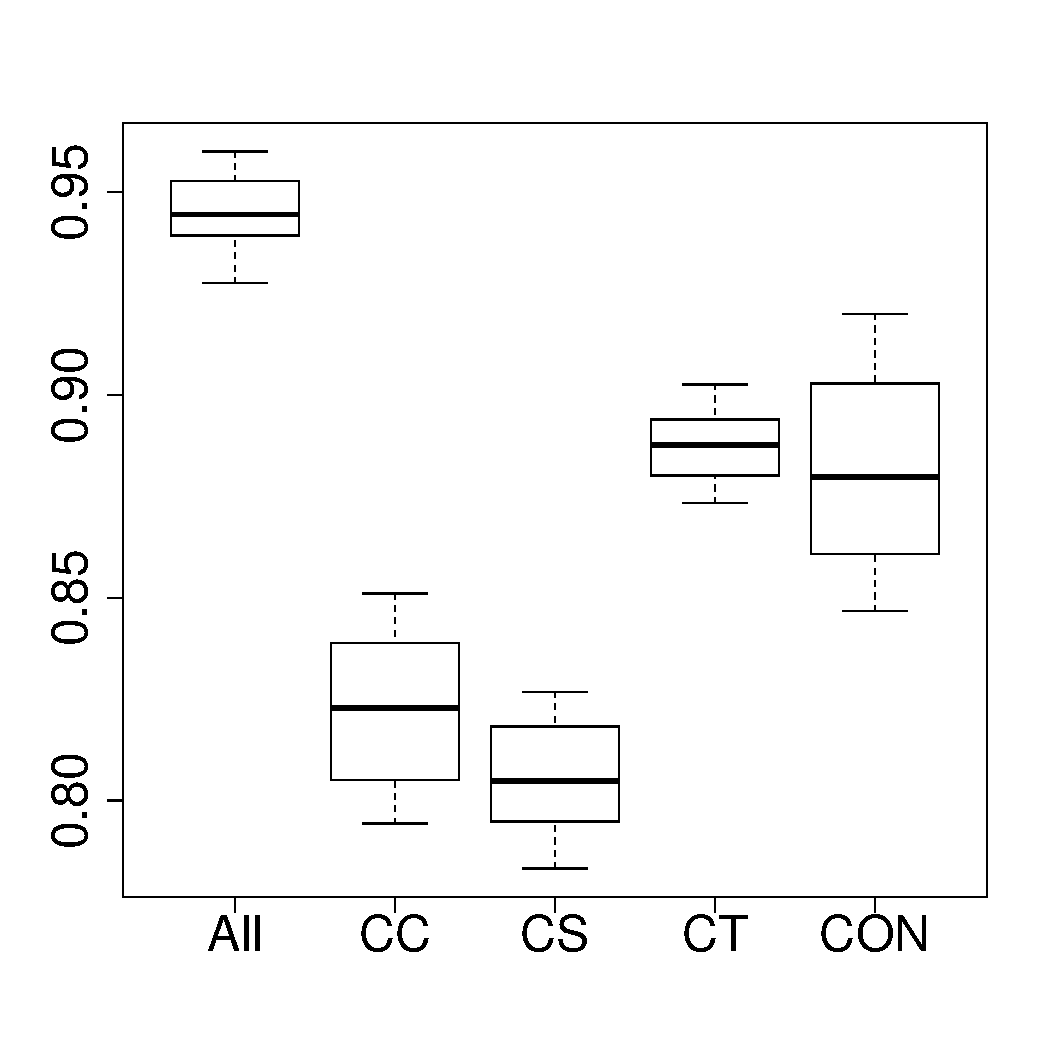
\includegraphics[width=\linewidth]{Figures/runtime-hadoopkeep-importance.pdf}
                \caption{Res. time}
        \end{subfigure}%
        \begin{subfigure}{0.19\textwidth}
                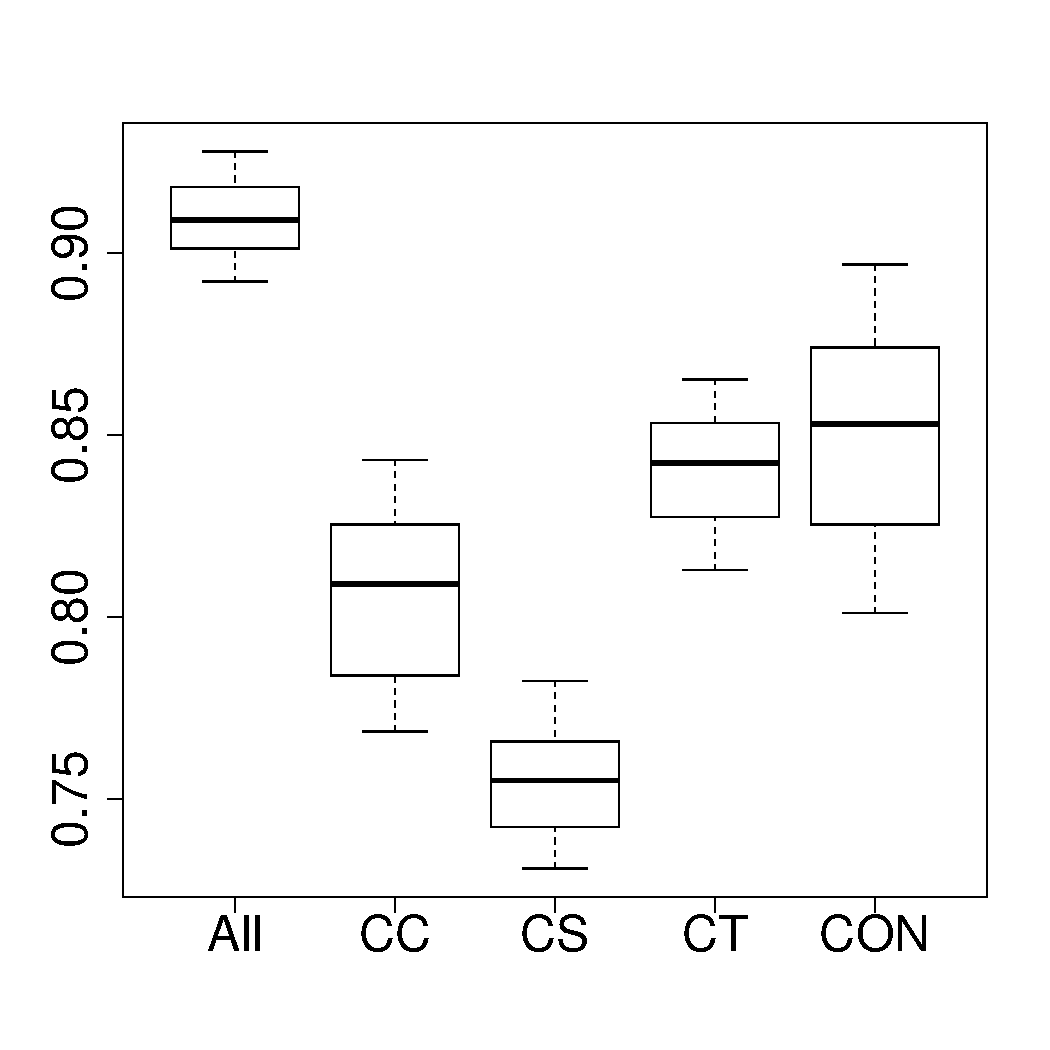
\includegraphics[width=\linewidth]{Figures/cpu-hadoopkeep-importance.pdf}
                \caption{CPU}
        \end{subfigure}%
        \begin{subfigure}{0.19\textwidth}
                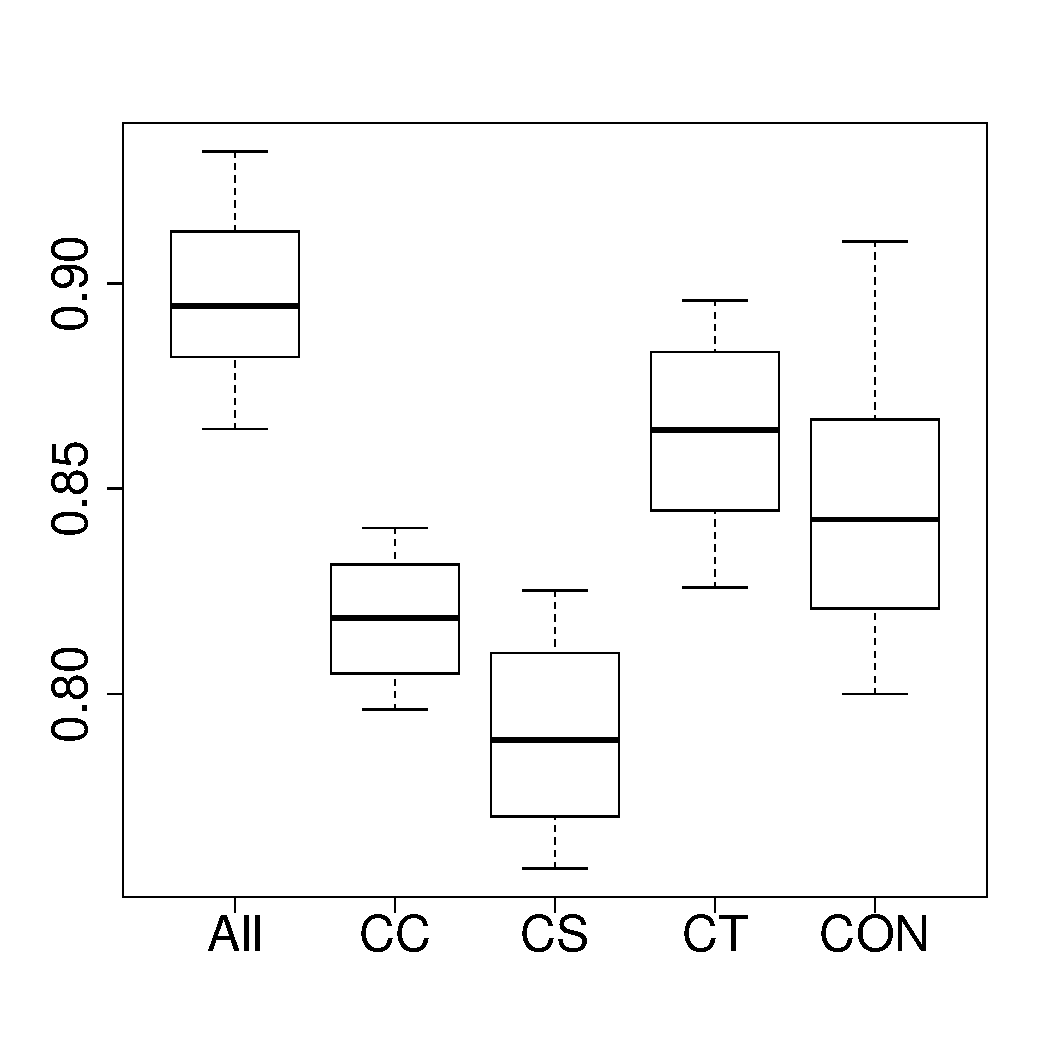
\includegraphics[width=\linewidth]{Figures/mem-hadoopkeep-importance.pdf}
                \caption{Memory}
        \end{subfigure}%
        \begin{subfigure}{0.19\textwidth}
                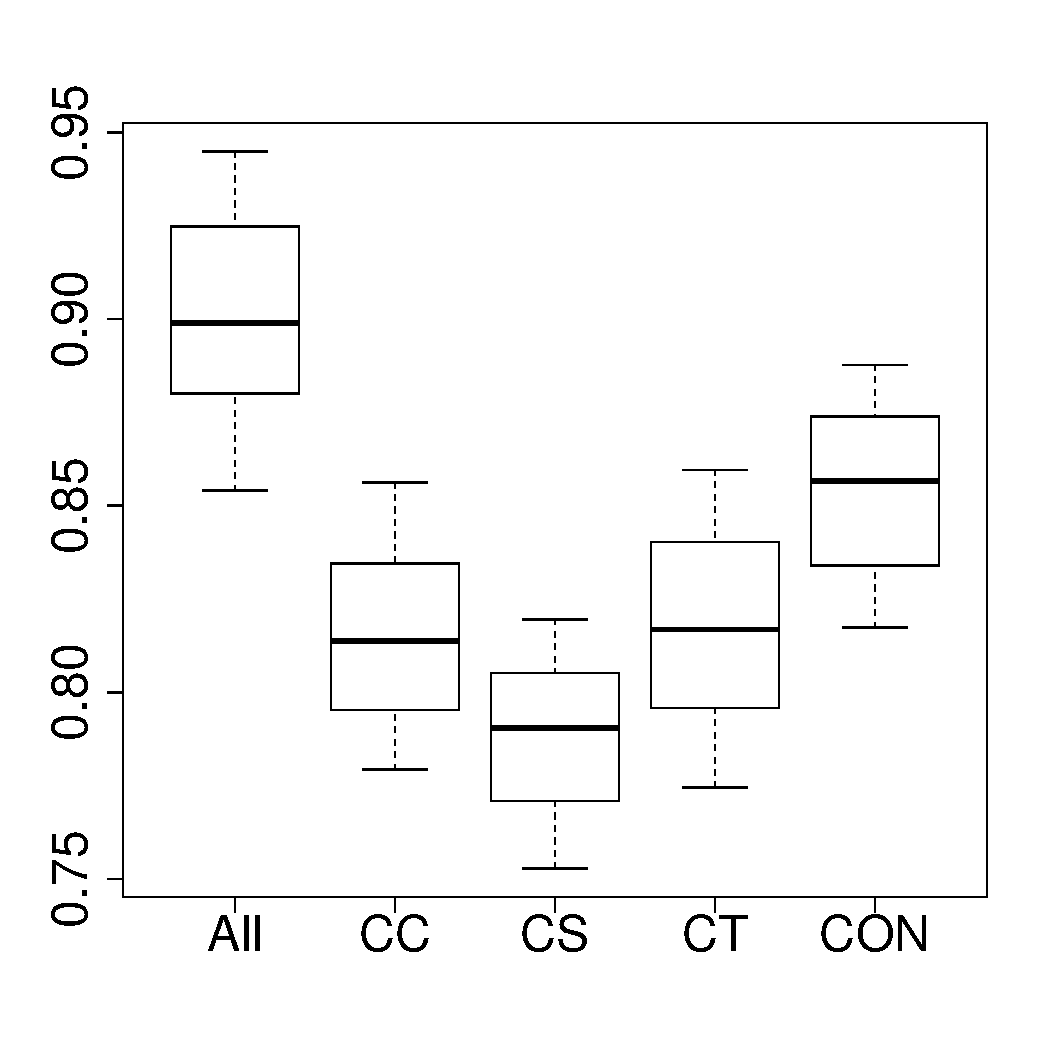
\includegraphics[width=\linewidth]{Figures/ioread-hadoopkeep-importance.pdf}
                \caption{I/O read}
        \end{subfigure}
        \begin{subfigure}{0.19\textwidth}
                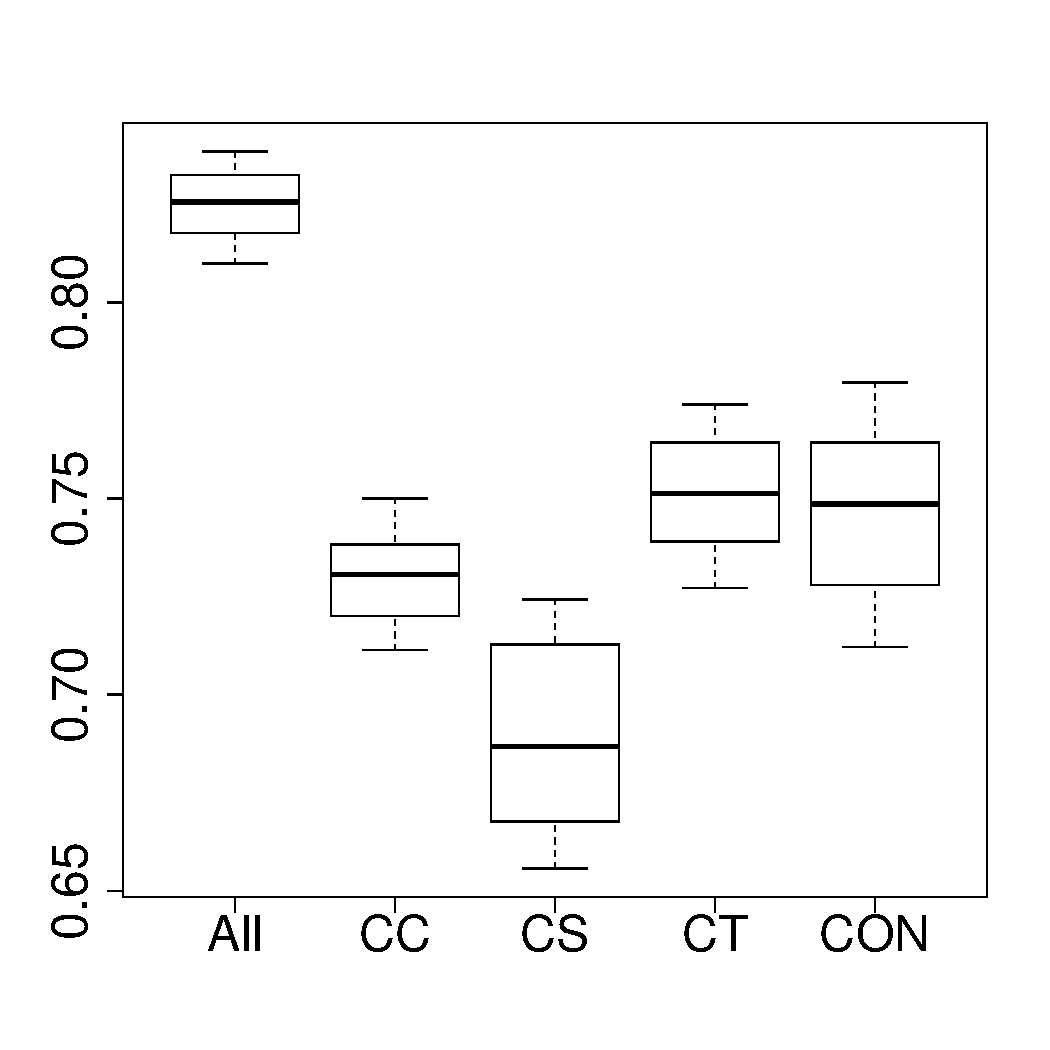
\includegraphics[width=\linewidth]{Figures/iowrite-hadoopkeep-importance.pdf}
                \caption{I/O write}
        \end{subfigure}
        
	\caption{AUC of RF for \emph{Hadoop} when only keeping one dimension of metrics.}
	\label{fig:importance-dimenssion-keep-hadoop}
\end{figure}

\begin{figure}[t]
	\centering
        \begin{subfigure}{0.19\textwidth}
                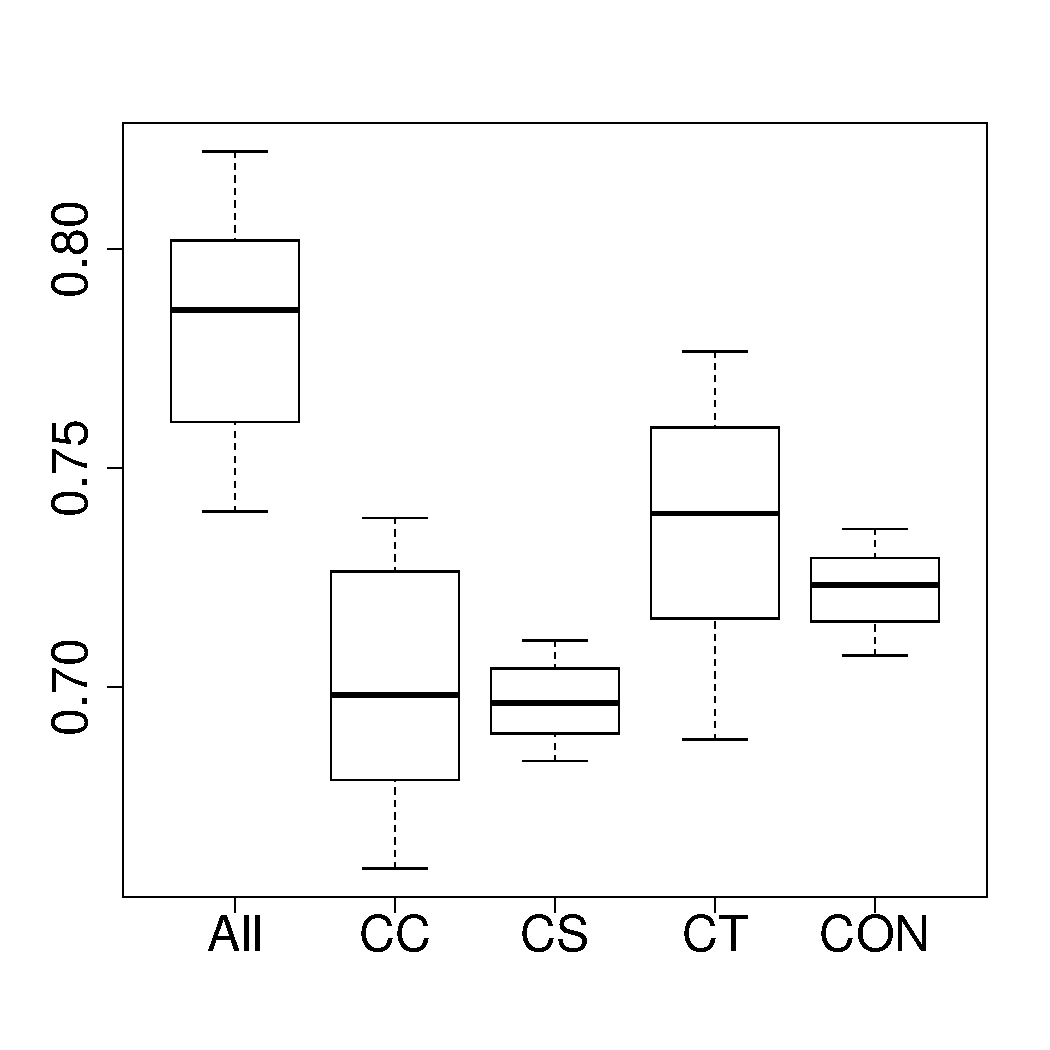
\includegraphics[width=\linewidth]{Figures/runtime-cassandrakeep-importance.pdf}
                \caption{Res. time}
        \end{subfigure}%
        \begin{subfigure}{0.19\textwidth}
                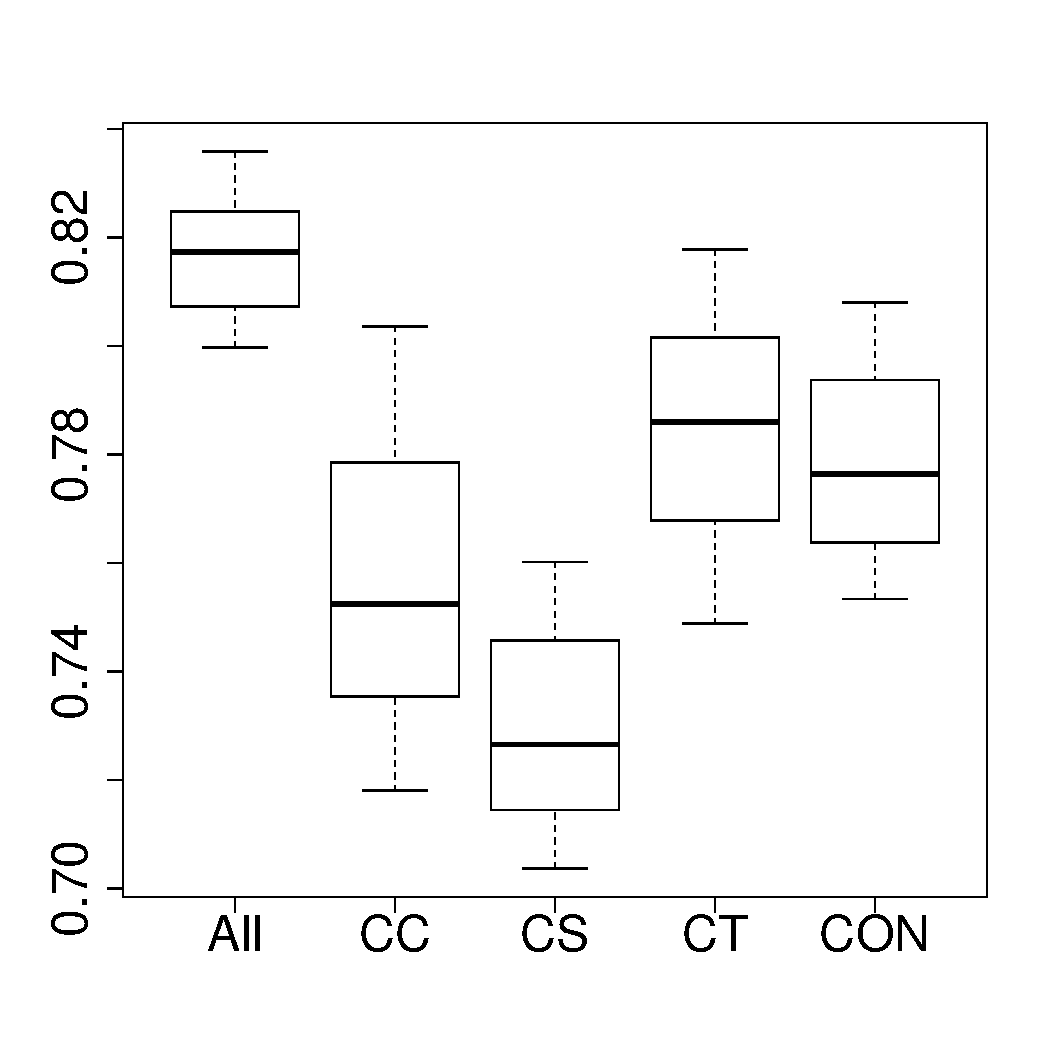
\includegraphics[width=\linewidth]{Figures/cpu-cassandrakeep-importance.pdf}
                \caption{CPU}
        \end{subfigure}%
        \begin{subfigure}{0.19\textwidth}
                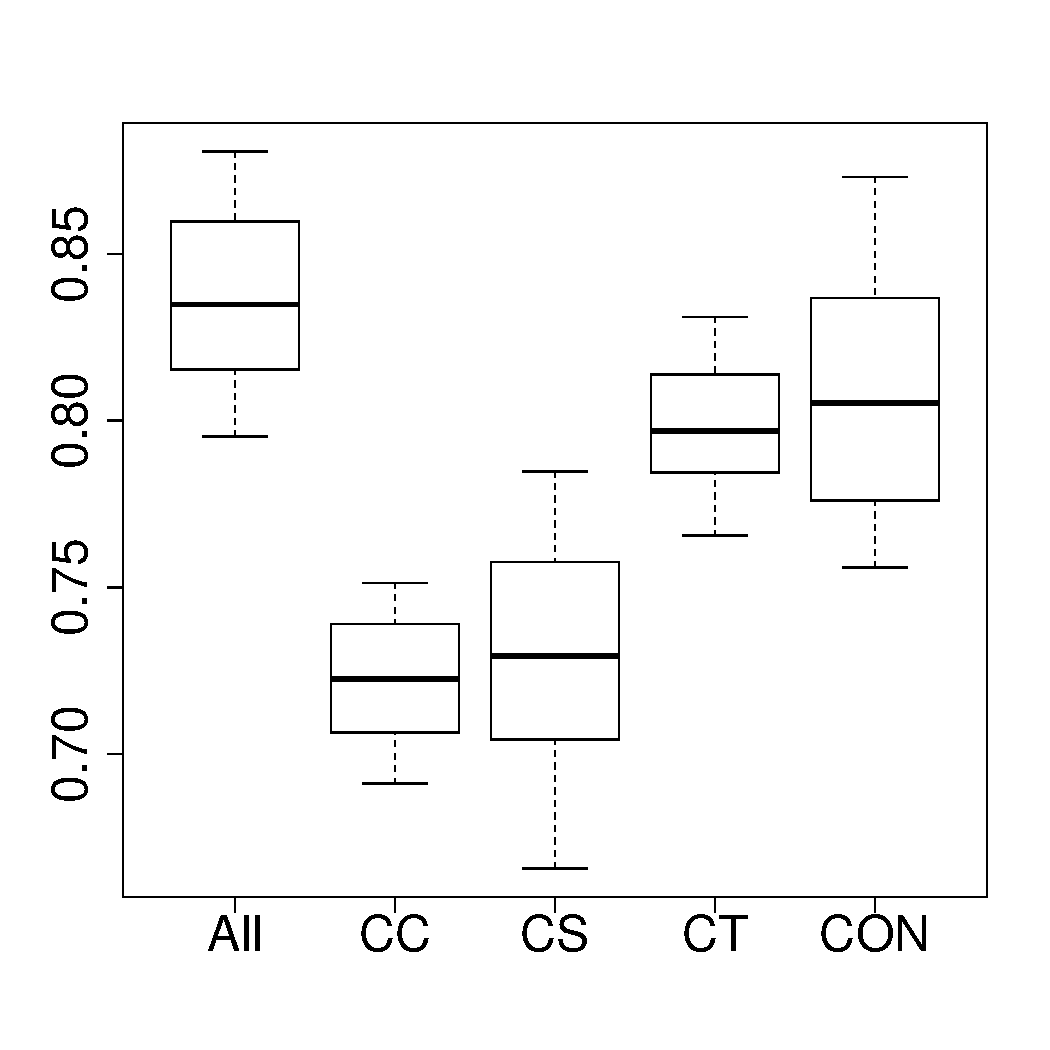
\includegraphics[width=\linewidth]{Figures/mem-cassandrakeep-importance.pdf}
                \caption{Memory}
        \end{subfigure}%
        \begin{subfigure}{0.19\textwidth}
                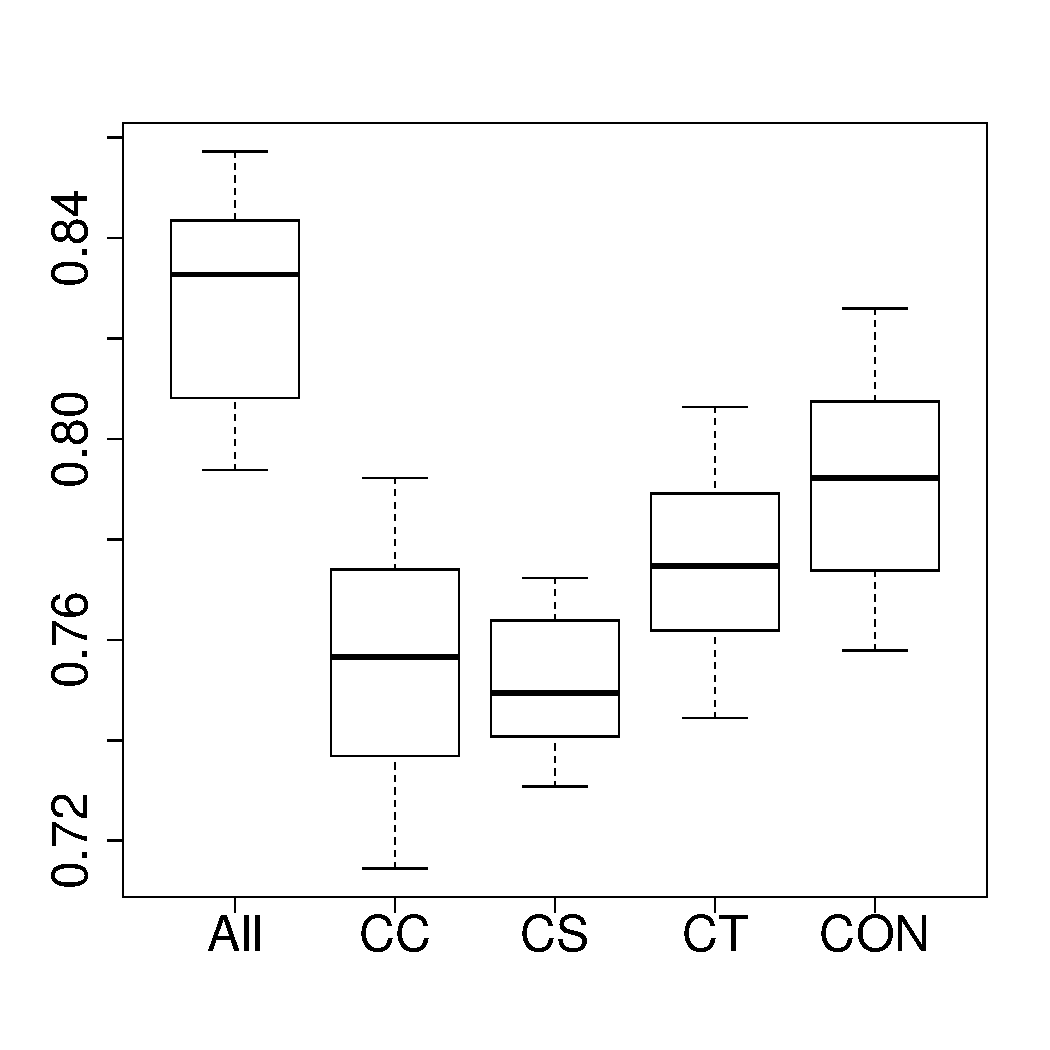
\includegraphics[width=\linewidth]{Figures/ioread-cassandrakeep-importance.pdf}
                \caption{I/O read}
        \end{subfigure}
        \begin{subfigure}{0.19\textwidth}
                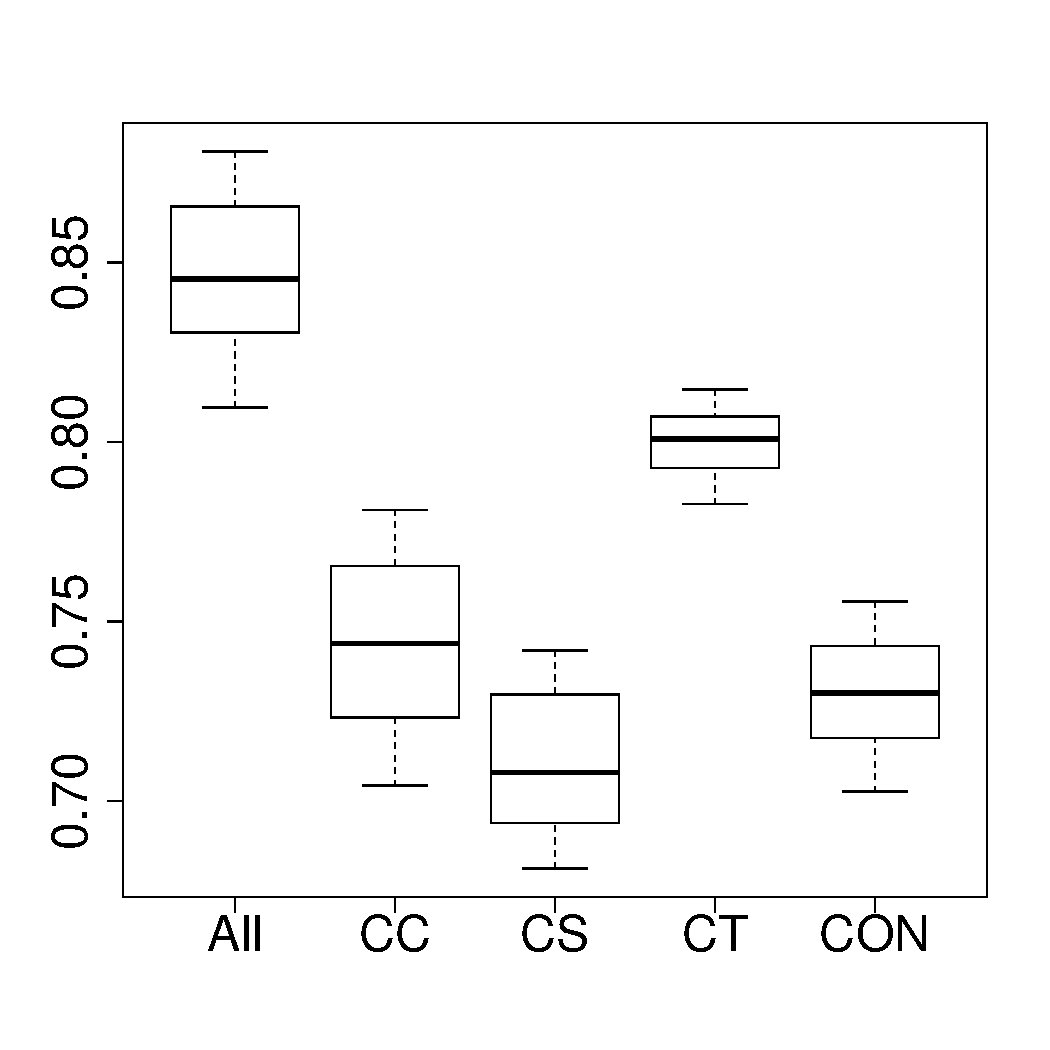
\includegraphics[width=\linewidth]{Figures/iowrite-cassandrakeep-importance.pdf}
                \caption{I/O write}
        \end{subfigure}
        
	\caption{AUC of RF for \emph{Cassandra} when only keeping one dimension of metrics.}
	\label{fig:importance-dimenssion-keep-cassandra}
\end{figure}

\begin{figure}[t]
	\centering
        \begin{subfigure}{0.19\textwidth}
                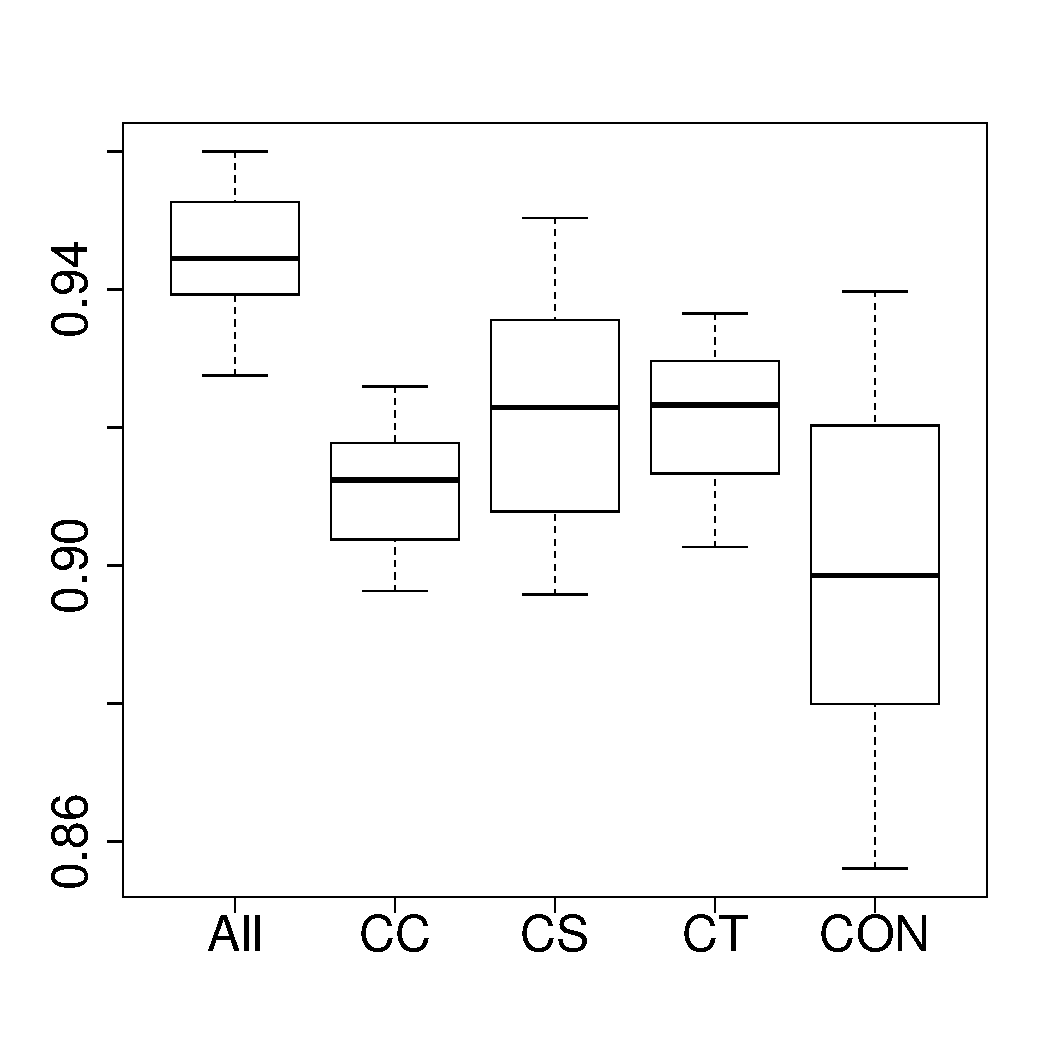
\includegraphics[width=\linewidth]{Figures/runtime-hadoopremove-importance.pdf}
                \caption{Res. time}
        \end{subfigure}%
        \begin{subfigure}{0.19\textwidth}
                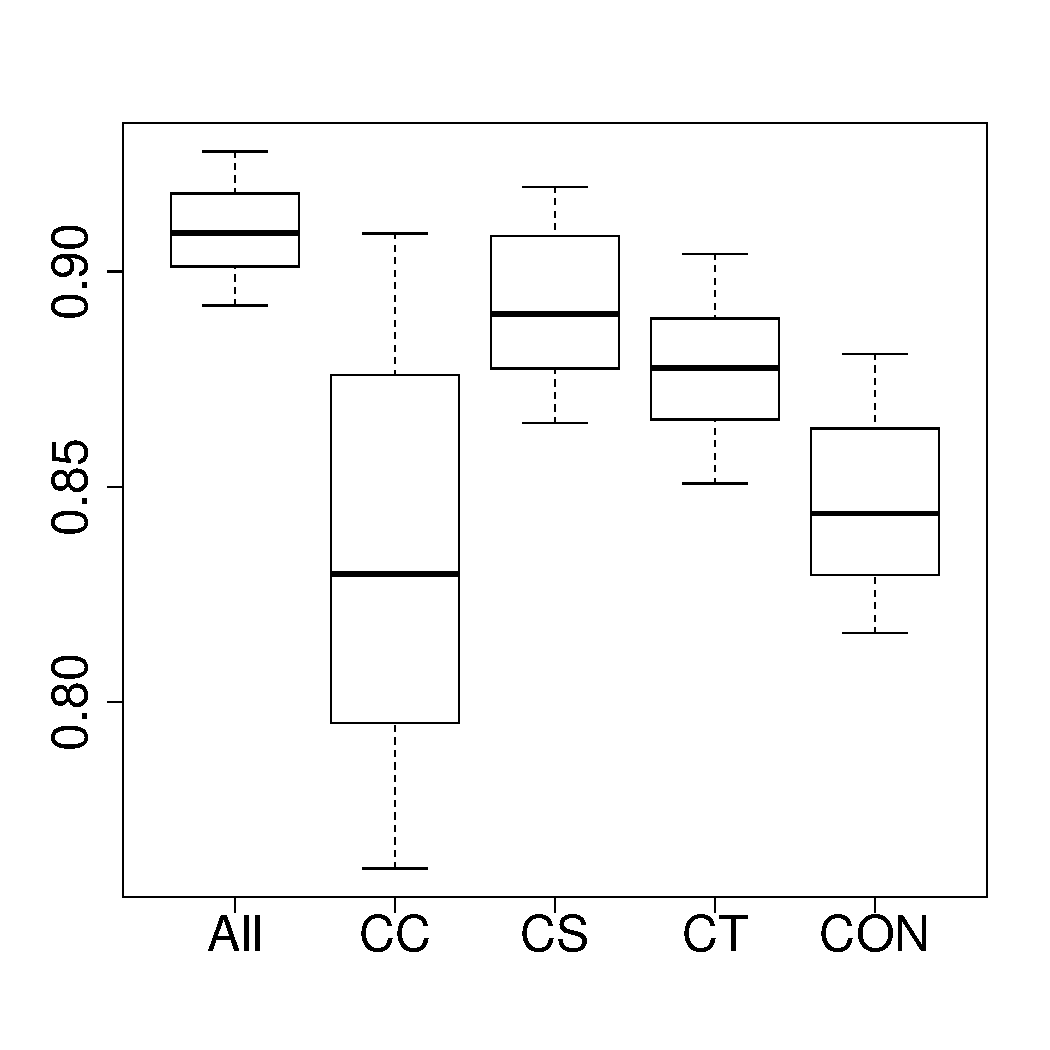
\includegraphics[width=\linewidth]{Figures/cpu-hadoopremove-importance.pdf}
                \caption{CPU}
        \end{subfigure}%
        \begin{subfigure}{0.19\textwidth}
                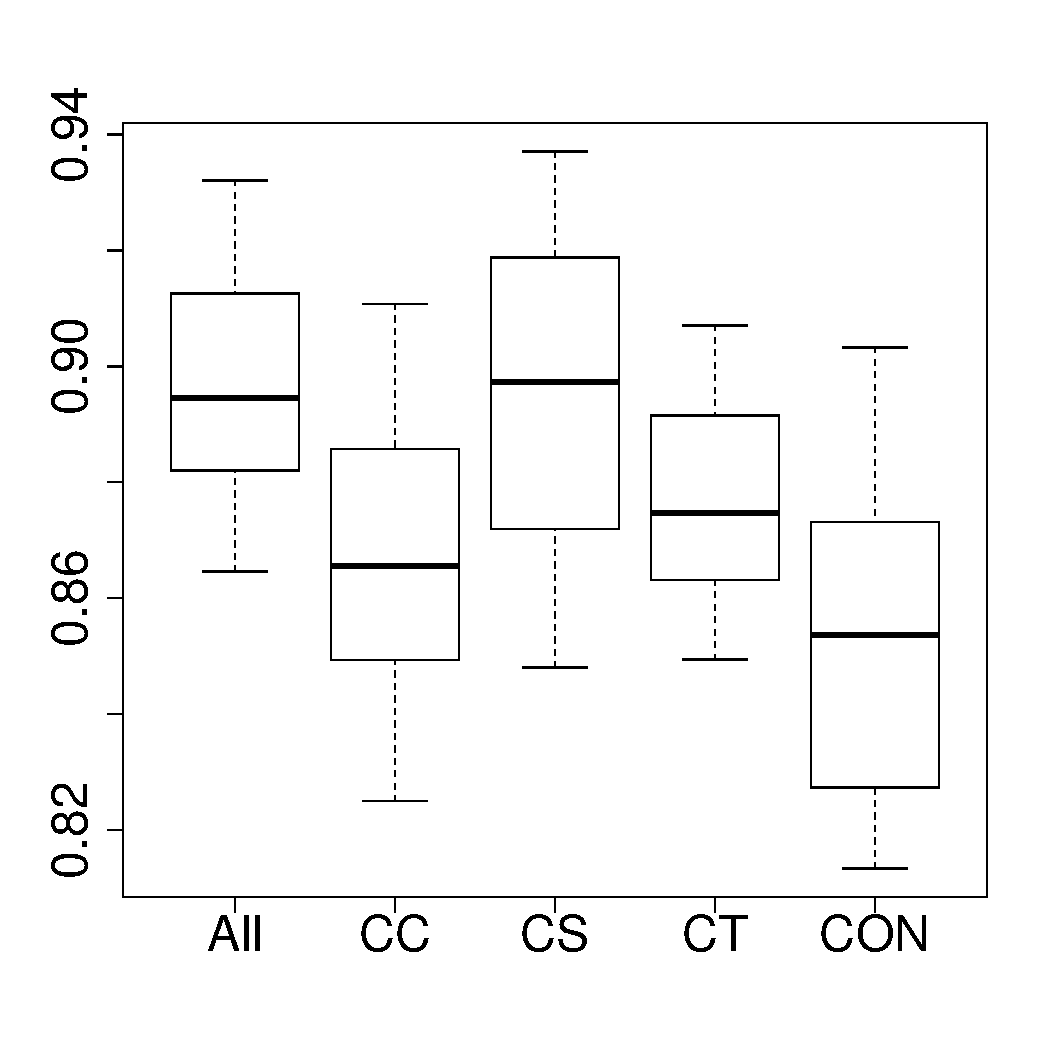
\includegraphics[width=\linewidth]{Figures/mem-hadoopremove-importance.pdf}
                \caption{Memory}
        \end{subfigure}%
        \begin{subfigure}{0.19\textwidth}
                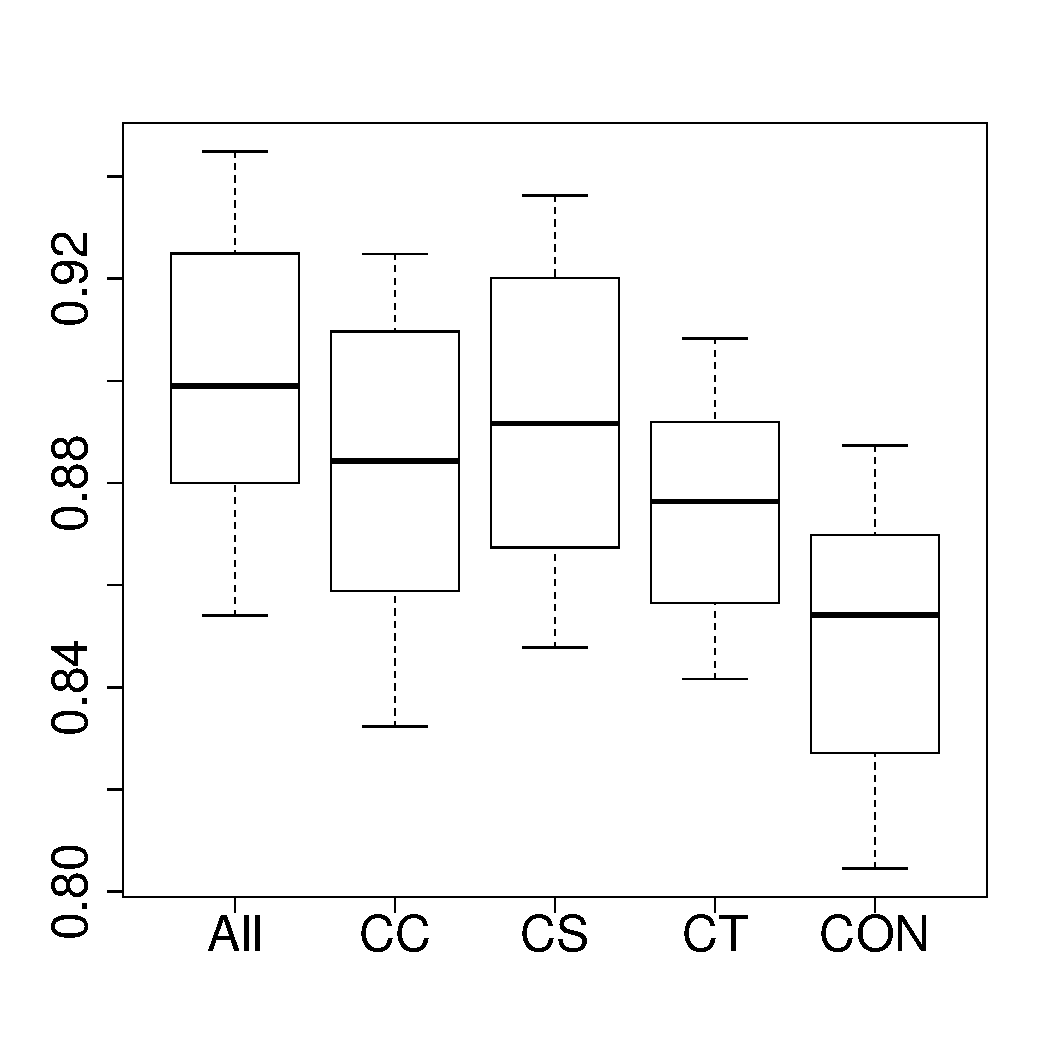
\includegraphics[width=\linewidth]{Figures/ioread-hadoopremove-importance.pdf}
                \caption{I/O read}
        \end{subfigure}
        \begin{subfigure}{0.19\textwidth}
                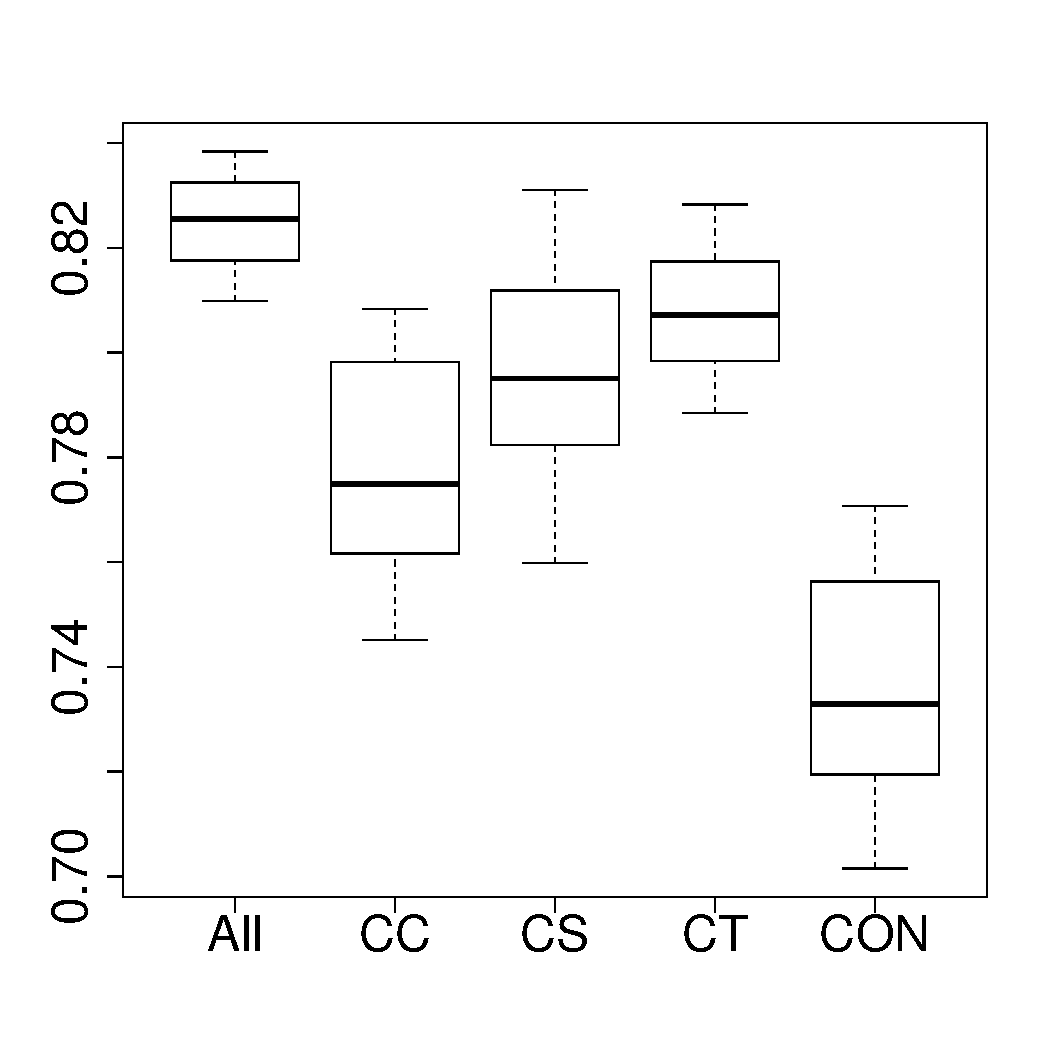
\includegraphics[width=\linewidth]{Figures/iowrite-hadoopremove-importance.pdf}
                \caption{I/O write}
        \end{subfigure}
        
	\caption{AUC of RF for \emph{Hadoop} when removing one dimension of metrics.}
	\label{fig:importance-dimenssion-remove-hadoop}
\end{figure}

\begin{figure}[t]
	\centering
        \begin{subfigure}{0.19\textwidth}
                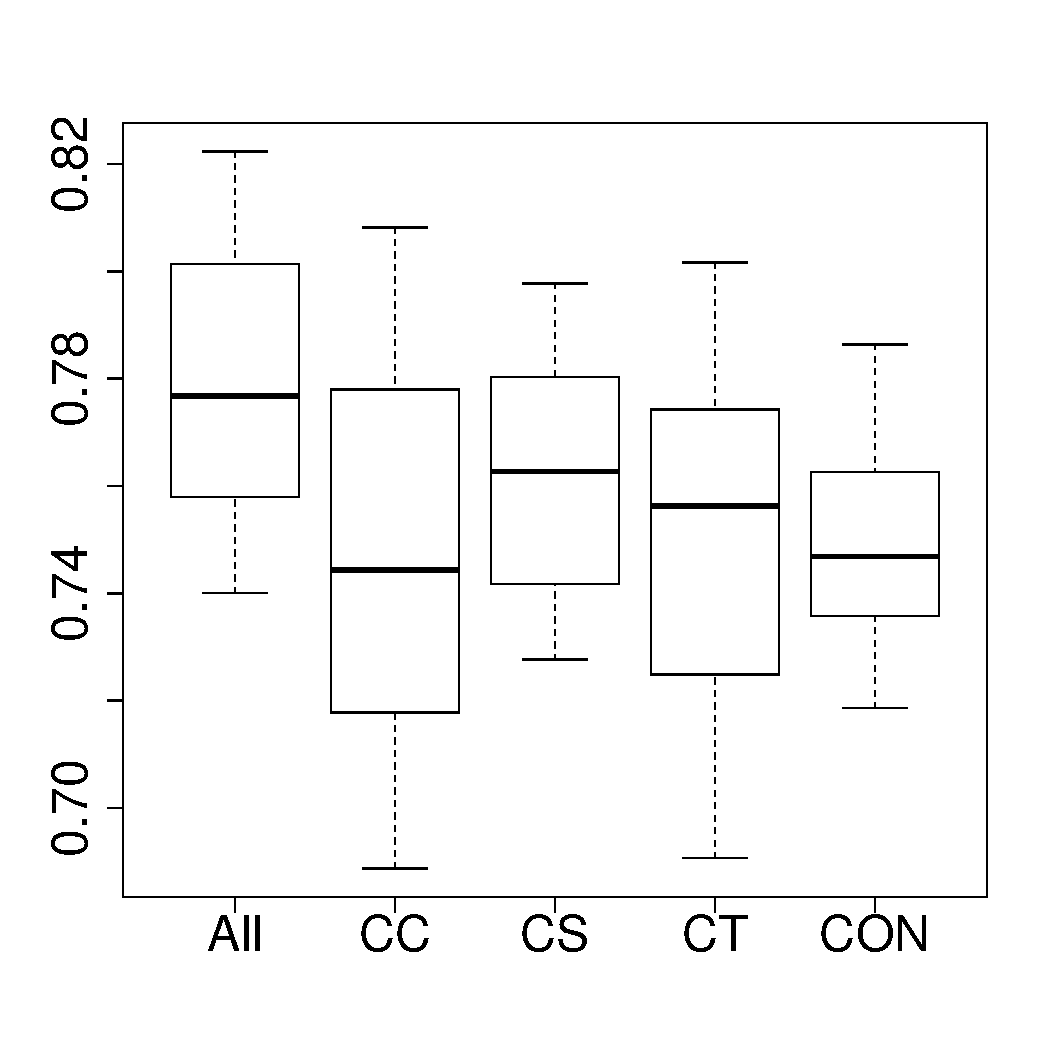
\includegraphics[width=\linewidth]{Figures/runtime-cassandraremove-importance.pdf}
                \caption{Res. time}
        \end{subfigure}%
        \begin{subfigure}{0.19\textwidth}
                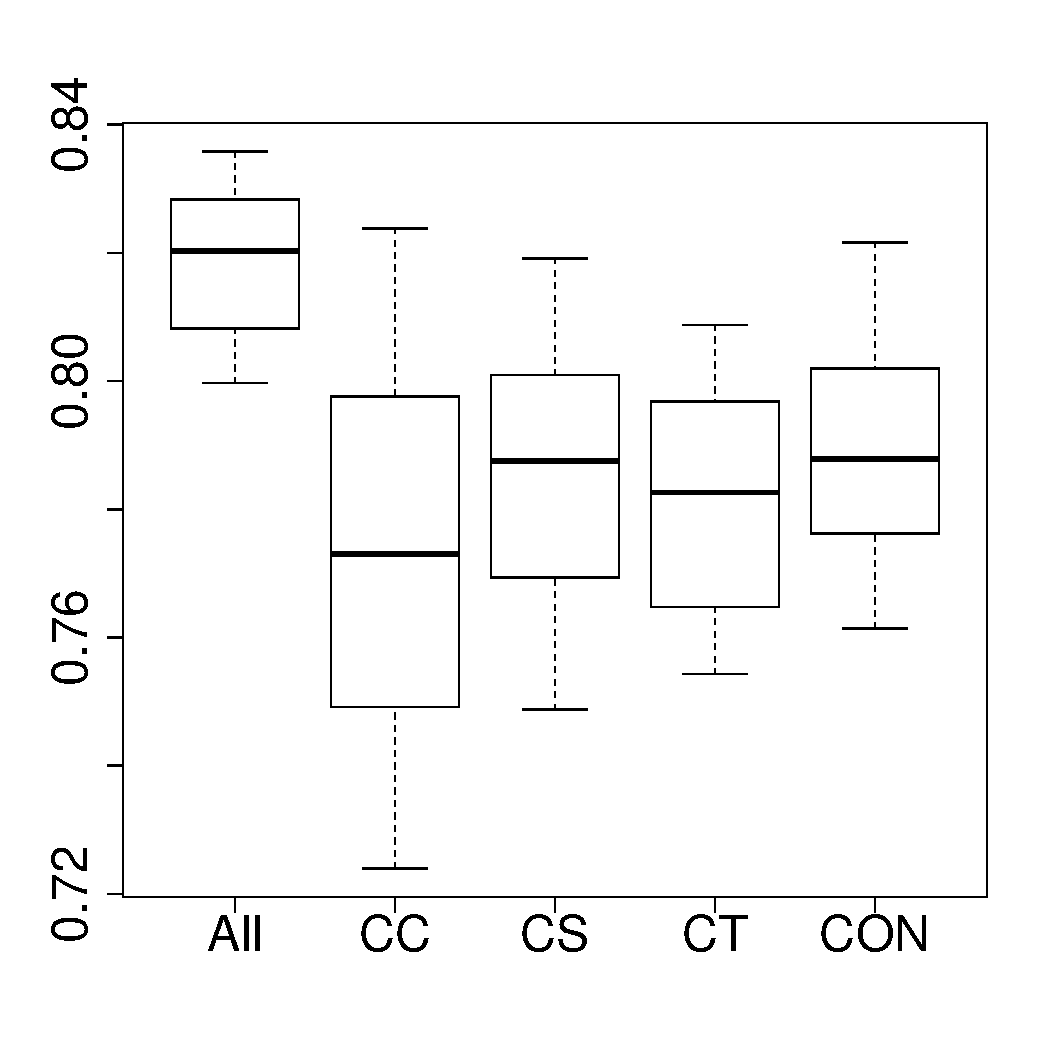
\includegraphics[width=\linewidth]{Figures/cpu-cassandraremove-importance.pdf}
                \caption{CPU}
        \end{subfigure}%
        \begin{subfigure}{0.19\textwidth}
                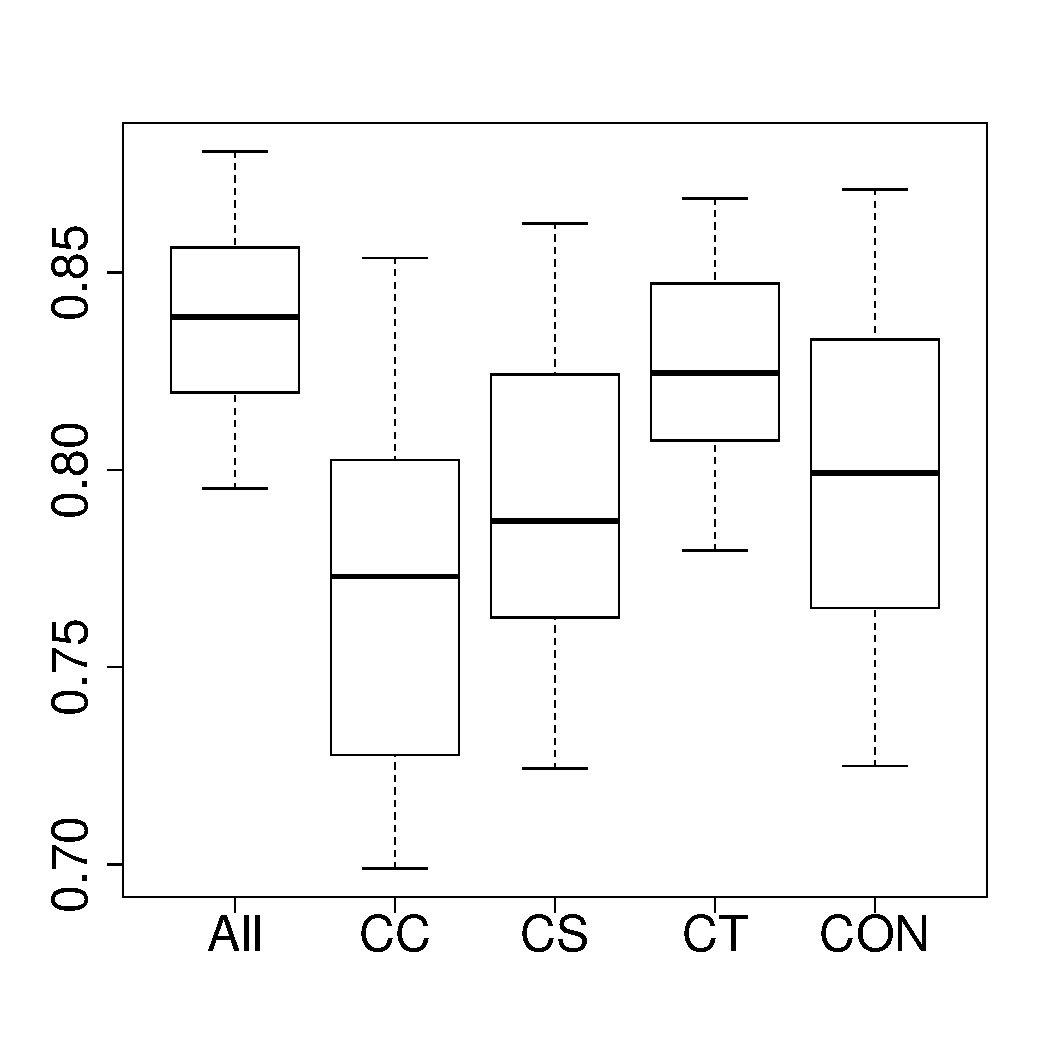
\includegraphics[width=\linewidth]{Figures/mem-cassandraremove-importance.pdf}
                \caption{Memory}
        \end{subfigure}%
        \begin{subfigure}{0.19\textwidth}
                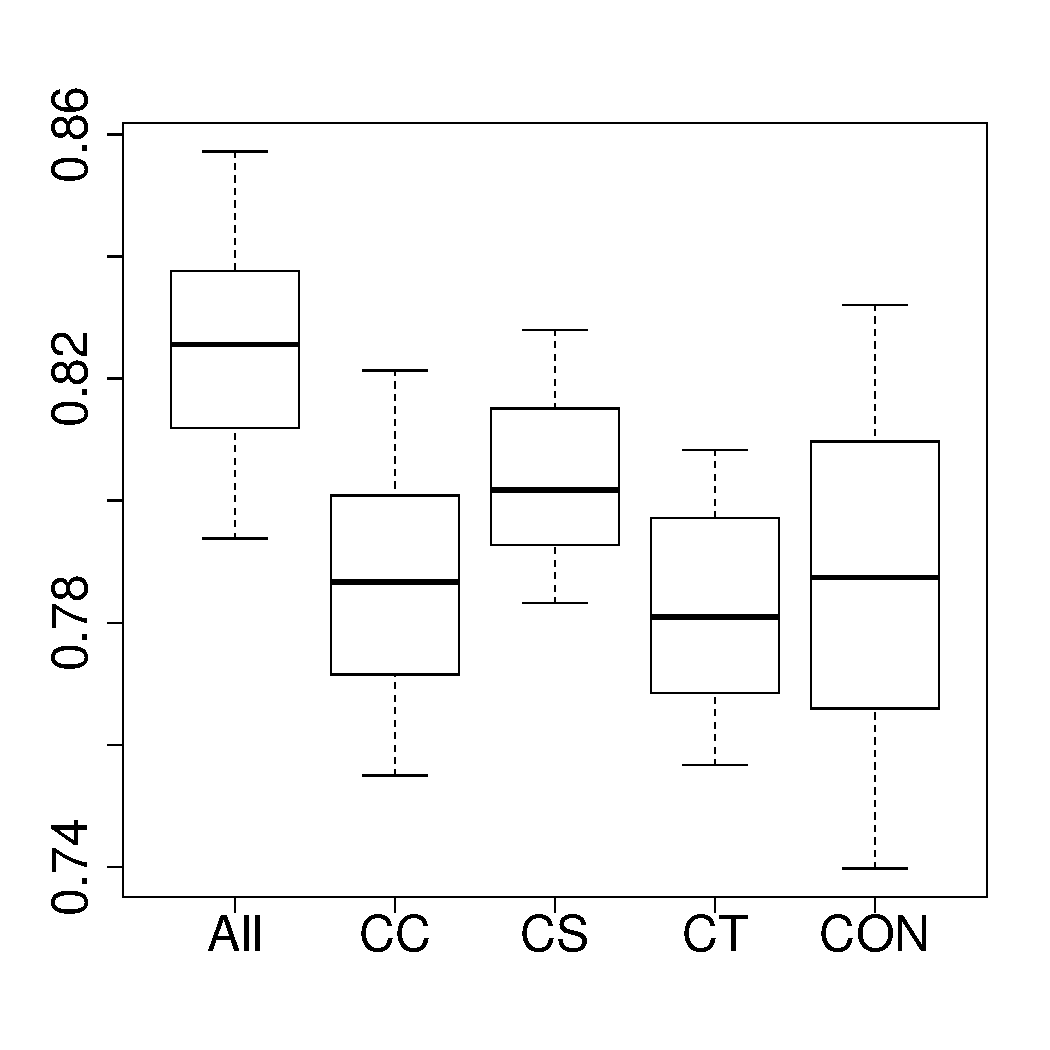
\includegraphics[width=\linewidth]{Figures/ioread-cassandraremove-importance.pdf}
                \caption{I/O read}
        \end{subfigure}
        \begin{subfigure}{0.19\textwidth}
                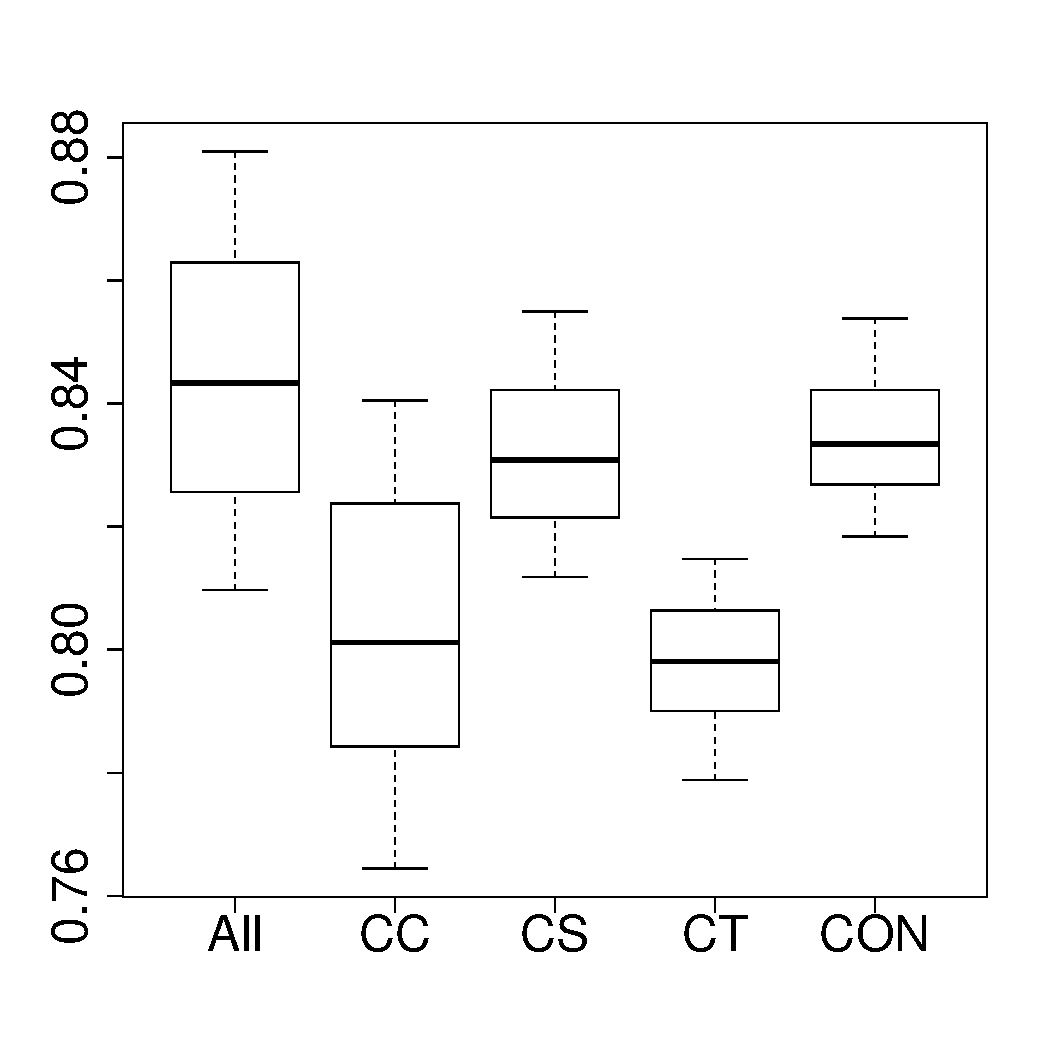
\includegraphics[width=\linewidth]{Figures/iowrite-cassandraremove-importance.pdf}
                \caption{I/O write}
        \end{subfigure}
        
	\caption{AUC of RF for \emph{Cassandra} when removing one dimension of metrics.} %\heng{the last box-plots have no label.} \heng{Make all the x/y labels bigger}}
	\label{fig:importance-dimenssion-remove-cassandra}
\end{figure}

%\noindent\textbf{All dimensions of metrics play important roles in our models, while the metrics may have different influence for different performance metrics and subject systems. } \heng{Test the significance of the difference between the models using all metrics and the models excluding one dimension of metrics. Alternative: use SK to rank the dimensions, including all metrics.}

%\noindent \textbf{\jinfu{Configuration and code token dimensions of metrics play more important roles in our model.}} The result of average AUC and AUC changes after removing each dimension of metrics is shown in Table~\ref{tab:dimension_importance}. 
%The results show that after removing each dimension of metrics, the AUC values decreases ranging from 0.02 to 0.09. The results of only keeping one dimension metrics is shown in Table~\ref{tab:one_dimension_importance}. The values of average AUC changes ranging from 0.04 to 0.14. Intuitively, the most important dimension metrics are the metrics from configuration dimension. %In particular, for \emph{Hadoop}, the average AUC value in configuration dimension decreases by 0.06 compared to the original model. The second most important dimension metrics is code change dimension metrics. 

%To examine whether there exist statistically significantly difference in AUC between original model and the resulting model, we apply e Mann-Whitney U test on our resulting AUC data. The result is shown in Table~\ref{tab:difference}. The results show that there exist statistically significant difference (p\_value  \textless  0.05) in the predictions between most of the dimension metrics and all metrics. Such results imply that any of dimension metrics play important roles in our models.



\begin{comment}

\med{to remove with table 10}\noindent\textbf{For the Hadoop project, the \textit{configuration option} dimension has the most top-ranked metrics; while for the Cassandra project, the \textit{code change} and \textit{code token} dimensions have the most top-ranked metrics.}
\med{not sure to understand this ->}As discussed in RQ1, the configuration options show more consistent influence on the performance regression detection in the Hadoop project than in the Cassandra project, which could explain that the configuration metrics are ranked higher in the Hadoop project. 
%\heng{Detailed examples of individual metrics and their meanings.}
The results of average rank of the top important individual metrics is shown in Table~\ref{tab:individual_importance}. For \emph{Hadoop}, the results show that the most important metric is the token named \emph{groups} in dimension configuration. For \emph{Cassandra}, the most important metric is \emph{Entropy} in dimension code change. 

\begin{table}
\tabcolsep=0.05cm
\tiny
\caption{Average rank of the top ten important metrics and their corresponding dimension.}

\begin{tabular}{|c|c|c|c|c|c|c|c|c|c|c|}
\hline
\multicolumn{11}{|c|}{Hadoop}                                                                                                                                                    \\ \hline
\multirow{2}{*}{Rank} & \multicolumn{2}{c|}{Res. Time} & \multicolumn{2}{c|}{CPU} & \multicolumn{2}{c|}{Memory} & \multicolumn{2}{c|}{I/O read} & \multicolumn{2}{c|}{I/O write} \\ \cline{2-11} 
                      & dimension    & metric          & dimension  & metric      & dimension      & metric     & dimension   & metric          & dimension    & metric          \\ \hline
1                     & config       & groups          & config     & groups      & Change    & Entropy    & config      & stream          & config       & groups          \\ \hline
2                     & config       & multipart       & config     & secs        & config         & groups     & Change      & Entropy         & config       & idlethreshold   \\ \hline
3                     & Change       & Entropy         & config     & after       & config         & stream     & config      & after           & config       & ipc             \\ \hline
4                     & config       & ipc             & config     & kill        & config         & secs       & config      & symlinks        & config       & after           \\ \hline
5                     & config       & zk              & Change     & Entropy     & config         & checksum   & config      & groups          & Change       & Entropy         \\ \hline
6                     & config       & secs            & config     & close       & token          & static     & config      & ipc             & config       & retries         \\ \hline
7                     & config       & authorization   & config     & checksum    & config         & symlinks   & config      & secs            & config       & secs            \\ \hline
8                     & token        & build           & config     & symlinks    & config         & after      & config      & authorization   & config       & checksum        \\ \hline
9                     & config       & checksum        & config     & stream      & config         & server     & config      & close           & config       & stream          \\ \hline
10                    & token        & builtin         & config     & tcpnodelay  & config         & kill       & config      & maxidletime     & config       & symlinks        \\ \hline
\multicolumn{11}{|c|}{Cassandra}                                                                                                                                                 \\ \hline
\multirow{2}{*}{Rank} & \multicolumn{2}{c|}{Res. Time} & \multicolumn{2}{c|}{CPU} & \multicolumn{2}{c|}{Memory} & \multicolumn{2}{c|}{I/O read} & \multicolumn{2}{c|}{I/O write} \\ \cline{2-11} 
                      & dimension    & metric          & dimension  & metric      & dimension      & metric     & dimension   & metric          & dimension    & metric          \\ \hline
1                     & Change       & Entropy         & Change     & Entropy     & Change         & Entropy    & Change      & Entropy         & Change       & Entropy         \\ \hline
2                     & Structure    & Fanin           & Structure  & Fanin       & Structure      & Fanin      & Structure   & Fanin           & Structure    & Fanin           \\ \hline
3                     & Change       & SOCM            & Change     & NS          & Change         & NS         & Change      & NS              & token        & cql             \\ \hline
4                     & token        & cql             & Change     & SOCM        & Change         & SOCM       & token       & get             & Change       & NS              \\ \hline
5                     & Change       & NS              & token      & metadata    & token          & get        & Change      & SOCM            & Change       & SOCM            \\ \hline
6                     & token        & get             & token      & equal       & token          & t          & token       & metadata        & token        & get             \\ \hline
7                     & Change       & SUMC            & token      & get         & token          & metadata   & token       & kei             & Change       & SUMC            \\ \hline
8                     & token        & metadata        & token      & kei         & token          & equal      & Change      & SUMC            & token        & metadata        \\ \hline
9                     & config       & failure         & Change     & SUMC        & token          & kei        & token       & in              & token        & d               \\ \hline
10                    & token        & kei             & config     & failure     & token          & size       & token       & store           & token        & kei             \\ \hline
\end{tabular}

\label{tab:individual_importance}
\end{table}


\end{comment}


\vspace{0.5cm}
\begin{Summary}{Summary of RQ2}{}
Every dimension of metrics plays an statistically significant role in predicting whether a \instance manifests a \inconsistent problem. The most important dimensions are related to code tokens and configurations. 
\end{Summary}
